\documentclass[11pt, tikz]{standalone}
\usepackage[T1]{fontenc}
\usepackage[utf8]{inputenc}
%\usepackage{textcomp}
%\renewcommand{\ttdefault}{lmtt} % 
\usepackage{amsmath}
\usetikzlibrary{arrows.meta, decorations.pathmorphing, positioning, calc}
\usepackage{xcolor}
\usepackage{amssymb,amsmath}

\begin{document}\sffamily
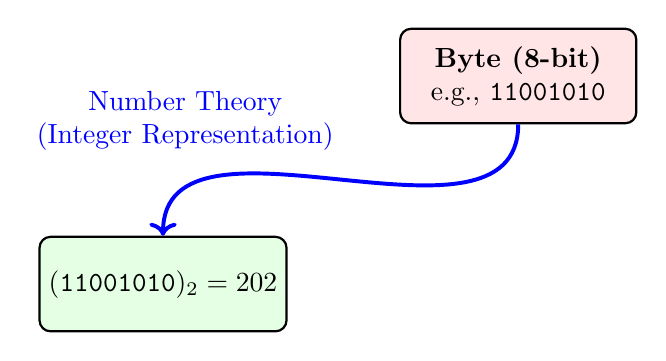
\begin{tikzpicture}[
	bluebox/.style={rectangle, draw, thick, rounded corners, minimum height=1.2cm, minimum width=2.5cm, align=center, fill=blue!10},
	yellowbox/.style={rectangle, draw, thick, rounded corners, minimum height=1.2cm, minimum width=2.5cm, align=center, fill=yellow!10},
	greenbox/.style={rectangle, draw, thick, rounded corners, minimum height=1.2cm, minimum width=3cm, align=center, fill=green!10},
	redbox/.style={rectangle, draw, thick, rounded corners, minimum height=1.2cm, minimum width=3cm, align=center, fill=red!10},
	arrow/.style={->, line width=.5mm},
	every node/.style={align=center}
	]
	\node[redbox] (crypto-sw) {\textbf{Byte (8-bit)}\\ e.g., \texttt{11001010}};
	\node[greenbox, below left=2cm of crypto-sw] (ef) {$(\texttt{11001010})_2=202$};
%	\node[greenbox, below=4cm of crypto-sw] (fc) {$\texttt{11001010}=(0,1,0,1,0,0,1,1)\in\mathbb{F}_2^8$};
%	\node[greenbox, below right=2cm of crypto-sw,align=center] (sca) {$\texttt{11001010}=x^7+x^6+x^3+x$ over\\ $GF(2^8)=\mathbb{F}_2[x]/\langle x^8+x^4+x+1\rangle$};
	
	\draw[arrow, blue, out=-90, in=90] (crypto-sw) to (ef);
	\node[blue, below left=1cm of crypto-sw, yshift=1.25cm, align=center] () {Number Theory\\ (Integer Representation)};
	
%	\draw[arrow, blue, out=-90, in=90] (crypto-sw) to (sca);
%	\node[blue, below=2cm of crypto-sw, xshift=1.25cm] () {Linear Algebra\\ (Vector Space)};
%	
%	\draw[arrow, blue, out=-90, in=90] (crypto-sw) to (fc);
%	\node[blue, below right=1cm of crypto-sw, yshift=1.25cm] () {Abstract Algebra\\ (Polynomial, Finite Field)};
	
%	\draw[dotted, <->, line width=.5mm, red, out=-90, in=180] (ef) to (fc);
%	\draw[dotted, <->, line width=.5mm, red, out=0, in=-90] (fc) to (sca);
\end{tikzpicture}
\end{document}
